%!TEX root = ../PhDthesis.tex
\chapter{Reproducible science and visualization}

Although the subject of this thesis is centered around modeling of the
visual cortex, a reproducible workflow is crucial to all scientific
disciplines and especially so in the computational sciences. As part
of the work presented in this thesis, we describe a new workflow to
make the exploration, analysis and publication of complex models
easier and more reproducible at every step. In particular this chapter
describes how the HoloViews library developed to aid the work as part
of the PhD achieves these goals and provides a general solution to
data visualization, storage and analysis that is now used in a number
of research projects. Every result in this thesis was generated using
this workflow and a fully reproducible record of the work is available
at \url{thesis.philippjfr.com}.

Developing such a workflow was essential to allow quick exploration of
the highly non-linear models developed as part of this
research. Specifically, when dealing with complex models with a large
number of parameters, which also evolve over time, existing tools were
not suited for the job. This is because a major component of this work
and work in other fields is an iterative process exploring some
parameter space, gaining insight into the behavior of the model and
then refining the model with the insights gained by careful
analysis. For this purpose we present a workflow, starting with the
declaration of a parameter space to explore, demonstrating how the
simulations can easily be launched locally or on a distributed cluster
and then be collected together for analysis. Finally we demonstrate
how the HoloViews library lets you load the data as it is generated,
monitor the progress, and then provides powerful tools to visualize and
analyze the resulting data up to and including publication-quality
figures.

We will begin by outlining the overall workflow and the philosophy
behind the individual components, before providing a case study on
the usage of the workflow as employed in this thesis.

\section{HoloViews: Building Complex Visualizations Easily for Reproducible Science}

One of the major contributions developed as part of this thesis is
development of the HoloViews data analysis and visualization library.
The library was developed to support this research in collaboration
with Jean-Luc Stevens and was published by Jean-Luc Stevens and myself
as joint first authors in the SciPy Conference Proceedings
\citep{Stevens2015}. Since then the library has become a popular
open-source library used in a wide range of scientific
disciplines. This section will outline the core design principles
behind HoloViews before applying it to a case study taken from one of
the results sections.

\subsection{Motivation}

In modern data analysis in scientific and engineering fields there is
often significantly more data available than a researcher can easily
review using standard plotting tools, in particular when the data is
dependent on a large number of variables, which cannot easily be
represented by the standard 2D or 3D plot types. The other barrier to
exploring these kind of datasets is that most plotting libraries are
not very well suited towards interactive analysis. The process of
visualizing is usually one that requires a lot of back and forth
between writing custom plotting code, viewing the results, and then
customizing the plot or writing more plotting code to view the data in
a different way. All this back and forth between the code and what the
researcher actually wants to do, which is to view the data, can kill
productivity and is a major obstacle in analyzing complex
datasets. Furthermore, it results in a disjointed, inefficient
workflow, accumulating custom code, which has to be maintained and
often becomes unreproducible.

HoloViews solves these fundamental problems by making the data
immediately visualizable. Unlike standard plotting approaches, the data
is always available on HoloViews objects. Thus a plot does not become a
dead end; each piece of data is annotated with the appropriate
metadata so it can be composed and processed into further
plots. Further, HoloViews objects can easily be converted between each
other, allowing very quickly iterating over different
visualizations. Finally HoloViews makes interactivity central to the
workflow---data with higher dimensionality than can be meaningfully
represented on a simple plot can be explored through interactive
sliders or by laying the data out in complex but highly informative
faceted plots.

HoloViews also improves the reproducibility of the results because
dependency on external plotting code is massively reduced, the
metadata is tightly coupled with the actual data, and HoloViews'
declarative style provides a readable description of what exactly is
being plotted. Next we will highlight the core design principles of
HoloViews that makes it so powerful as a tool for analysis,
visualization and publication.

\subsection{Design Principles}

The overriding design principle of HoloViews that the user should not
have to write a complex recipe of how they want their data to be
displayed.  Instead, HoloViews provides a set of declarative
data structures, which allow annotating the data with a minimal amount
of metadata to display a visual representation automatically and
transparently---the data should simply reveal itself.

The second core principle of HoloViews is that there should be a very
clear distinction between the details of visualization and actual data
and metadata required to describe a dataset. This means that the
atomic data objects (or Elements) should be very lightweight wrappers
around the actual data structure, along with a small amount of semantic
metadata. This allows creating, working with and storing the data
independent of the plotting code or any concerns about the visual
aesthetics of the plots.

The third design goal is the composability of the Elements. By
ensuring that different components can easily be composed together it
becomes very easy to build even complex plot types from simple
components. HoloViews provides operators and methods to make
overlaying and composing plots in layouts and grids very
straightforward.

These three guiding philosophies make HoloViews into an extremely
powerful tool to explore complex datasets easily while also providing
the flexibility to generate publication quality figures. In the next
section we will outline how this fits into an overall workflow and
demonstrate what these principles mean in practice. For a more in
depth review of the philosophy and principles behind the library refer
to the HoloViews paper in Appendix \ref{SciPyPaper}.

% Insert reference to HoloViews paper and to the appendix

\subsection{Contributions}

Since the \textsc{HoloViews} library was a joined project between
Jean-Luc Stevens it is important to delineate our contributions to the
library. The project was initially started as a way to explore the
temporally evolving models that was central to our research
approach. Soon after we came to realize the generality of the approach
and one of my major contributions was to push for a general system to
represent and explore data of any dimensionality and provide a system
not only to visualize the data but also apply basic statistical
operations on the data easily such as sampling and aggregating it.

Additionally my major contributions to the project were developing a
plotting backend for the bokeh interactive visualization library and
data backends for data analysis libraries such as pandas and
seaborn. Over the course of the project my contribution accounted for
around two thirds of all commits to the project and extended to every
aspect of the software.

\section{A unified workflow for the analysis of complex computational models}

When working with complex computational models or analyses it is often
necessary to launch large scale, parallel parameter explorations,
gather the results and apply analyses to the results. This often
involves separate scripts to launch the simulations and analysis
either locally and on a cluster and separate tools to gather this data
up from a shared storage location to visualize the results or apply
further analyses. This often results in collections of different
scripts and data files, which stitch together a disjointed workflow,
providing a serious barrier to reproducibility. As an alternative we
developed an integrated workflow based on the Lancet and HoloViews
libraries, which lets you trivially launch parameter explorations
either locally or on a cluster, monitor the progress and then lazily
load just the required subset of data for further analysis.

Through a concrete example we will explore how to specify each stage in
this analysis pipeline, highlighting the ease with which we can
launch, analyze and revise a model using this system. For this purpose
we will use a parameter exploration that is part of one of the results
chapters, skipping over the evaluation of the actual results for the
time being. While this is just one example, all the results produced
as part of this thesis are made available in the same format to
provide a fully reproducible record of the work done as part of this
project.

\subsection{The Jupyter notebook environment}

In order to generate truly reproducible research, it is not enough
simply to make sure that the analysis code is re-runnable. Instead,
one should guiding someone who is trying to reproduce the results through each
step so that they can not only replicate the results but also understand
each step and can begin modifying the workflow to take the
research further. This distinction separates mere replicability
from true reproducibility. In the past achieving this standard required documenting the
code and results meticulously in separate files, but even then this
workflow usually devolves into chaining script after script until the
workflow becomes difficult or impossible to follow for an external
researcher. The Jupyter notebook environment, spawned through the
IPython project \citep{Perez2007}, promises a solution to this problem,
by providing a platform that allows interleaving code with rich media
output and exposition, providing a detailed account of the steps
required to generate results and figures in a publication.

The entire workflow presented here is centered around the Jupyter
notebook, while not depending on it. It is what allows us to specify
an experiment to run, monitor progress, and present the results, all
accompanied by detailed exposition describing each stage. Each chapter
of this thesis will therefore be accompanied by one or more Jupyter
notebooks, which provide a fully reproducible account of how each
figure was generated, along with supplemental materials and results.

\subsection{Step 1: Specifying a parameter space}

The usual process of launching a parameter space analysis is to write
scripts to launch the jobs either locally or on a remote cluster. The
resulting files then have to be gathered up appropriately and should
preferably be accompanied by a log of the precise environment used to
launch the jobs. Lancet makes it trivial to specify jobs to execute
and will handle launching these jobs both locally and on a cluster,
keeping track of the files that were generated, the environment used
and any other extraneous information like version control data. In
\cite{Stevens2013a} the fundamental ideas behind Lancet are outlined
in detail, so here we will focus on how it integrates with the overall
workflow outlined in this chapter.

In this outline of the workflow we will be working with one of the
models that will be explored and developed as part of this thesis. To
get a better understanding of the model we want to vary multiple
parameters, apply measurements and analysis to the model, and then
evaluate the results. Defining the parameter space to explore is
incredibly straightforward. First we declare constant parameters, in
this case just the ``area`` of the model and the times in the
development of the model at which we want to apply measurements to the
model. Secondly we declare the varying parameters, in this case we
simply combine a ``Range`` of lateral excitatory strength
(``latexc\_strength``) with another ``Range`` of contrasts. The
multiplication operator automatically expands this parameter space by
taking the Cartesian product of the two varying sets of
parameters. Finally we combine the constant and varying parameters
into the overall parameter set for the batched experiment:

\begin{minipage}{\linewidth}
\begin{lstlisting}
times = [1000*i for i in range(21)]
constants = lancet.Args(area=3.0)
parameter_space = lancet.Range('latexc_strength', 0, 3.0, 11) * lancet.Range('contrast', 10, 100, 10)
batch_arguments =  constants * parameter_space * lancet.Args(times=times)
\end{lstlisting}
\end{minipage}

\subsection{Step 2: Specifying analysis}

Having defined the parameter space, the next step is defining the
actual model to run any measurements or analysis that are applied
to it. In this example we are working with the Topographica neural
simulator, which allows training large scale rate-based models on
visual input patterns. Here we load the SCAL model, which we will
present in the next chapter, and define a measurement of the
orientation map with subsequent analysis applied to the measured orientation
maps. This analysis will now be performed for each of the parameters
defined above, at each of the declared times. This approach makes it incredibly
easy to set up deferred execution of any number of measurements and
analyses, and even allows setting up complex chains of measurements and
analysis by declaring the output of one analysis as input to the next.

The ``Collector`` object will then apply the measurements at the times
defined as part of the parameter space, storing them as small
individual files, which can be loaded independently or all
together. Another benefit is that the Collector automatically records
the precise measurements that were defined, ensuring that the results
stay reproducible. Since the results are stored inside HoloViews
objects, they are instantly visualizable. All of these features ensure
that with very minimal effort by the user all the specifications to
set up the experiment are recorded, the results can easily be accessed,
and the entire process can easily be replicated from the logs that are
output by Lancet.


\begin{minipage}{\linewidth}
\begin{lstlisting}
  c = Collector()

  # Measurement
  c.collect(measure_or_pref, frequencies=[1.4, 1.6, 1.8])

  # Analysis
  c.Pinwheels.V1   = c.analyze(c.ref.OrientationPreference.V1 *\
                     c.ref.OrientationSelectivity.V1, PinwheelAnalysis)
  c.FFTAnalysis.V1 = c.analyze(c.ref.OrientationPreference.V1, PowerSpectrumAnalysis)
\end{lstlisting}
\end{minipage}

\subsection{Step 3: Launching jobs}

Having declared the parameter space we want to explore and what
exactly we want to measure, Lancet makes it trivial to launch the jobs
either locally or on a cluster, along with declarations about the
resources that each job should use. In most workflows this would
require distinct scripts for local and cluster execution. Using Lancet
you simply switch out the particular launcher that should be used. In
this case we declare that the jobs should be run on GridEngine via the
``QLauncher`` but simply by toggling QSUB to False we can switch to
local execution.

By providing this flexibility, the analysis and simulations can be
debugged locally and then trivially be executed on a cluster to launch
large-scale analyses or parameter explorations.

\begin{minipage}{\linewidth}
\begin{lstlisting}
  QSUB = True

  @lancet.review_and_launch()
  def launch():
      qsub_options = (b='y', pe=('sharedmem', '4'))
      launch_options = {'qsub_flag_optionsdict': qsub_options} if QSUB else {}
      runbatch_cmd = RunBatchCommand(ty_file, c, snapshot=False,
                                     metadata=batch_arguments.varying_keys)
      Launcher = lancet.QLauncher if QSUB else lancet.Launcher
      return Launcher(batch_name, batch_arguments, runbatch_cmd,
                    metadata=metadata(), **launch_options))
  launch()
\end{lstlisting}
\end{minipage}

\subsection{Step 4: Monitoring progress}

When launching large numbers of jobs it is important to keep track of
their progress to identify any problems and to ensure individual jobs
are actually completed. The modular file structure output by Lancet
can easily be loaded progressively, and using the live-interaction
features of HoloViews we can monitor the progress in real
time. Through various interactive tools it is easy to check on
individual jobs and find out which jobs are running slow or have
failed, so they can easily be relaunched if needed.

By building a simple dashboard using dynamic features in HoloViews, we
can keep track of the overall progress and each individual job.
We also provide tools to relaunch any jobs that fail to
complete. These features are crucial to keeping track of large numbers
of jobs, and ensure that the workflow is robust to various modes of
failure.

\begin{figure}
	\centering
        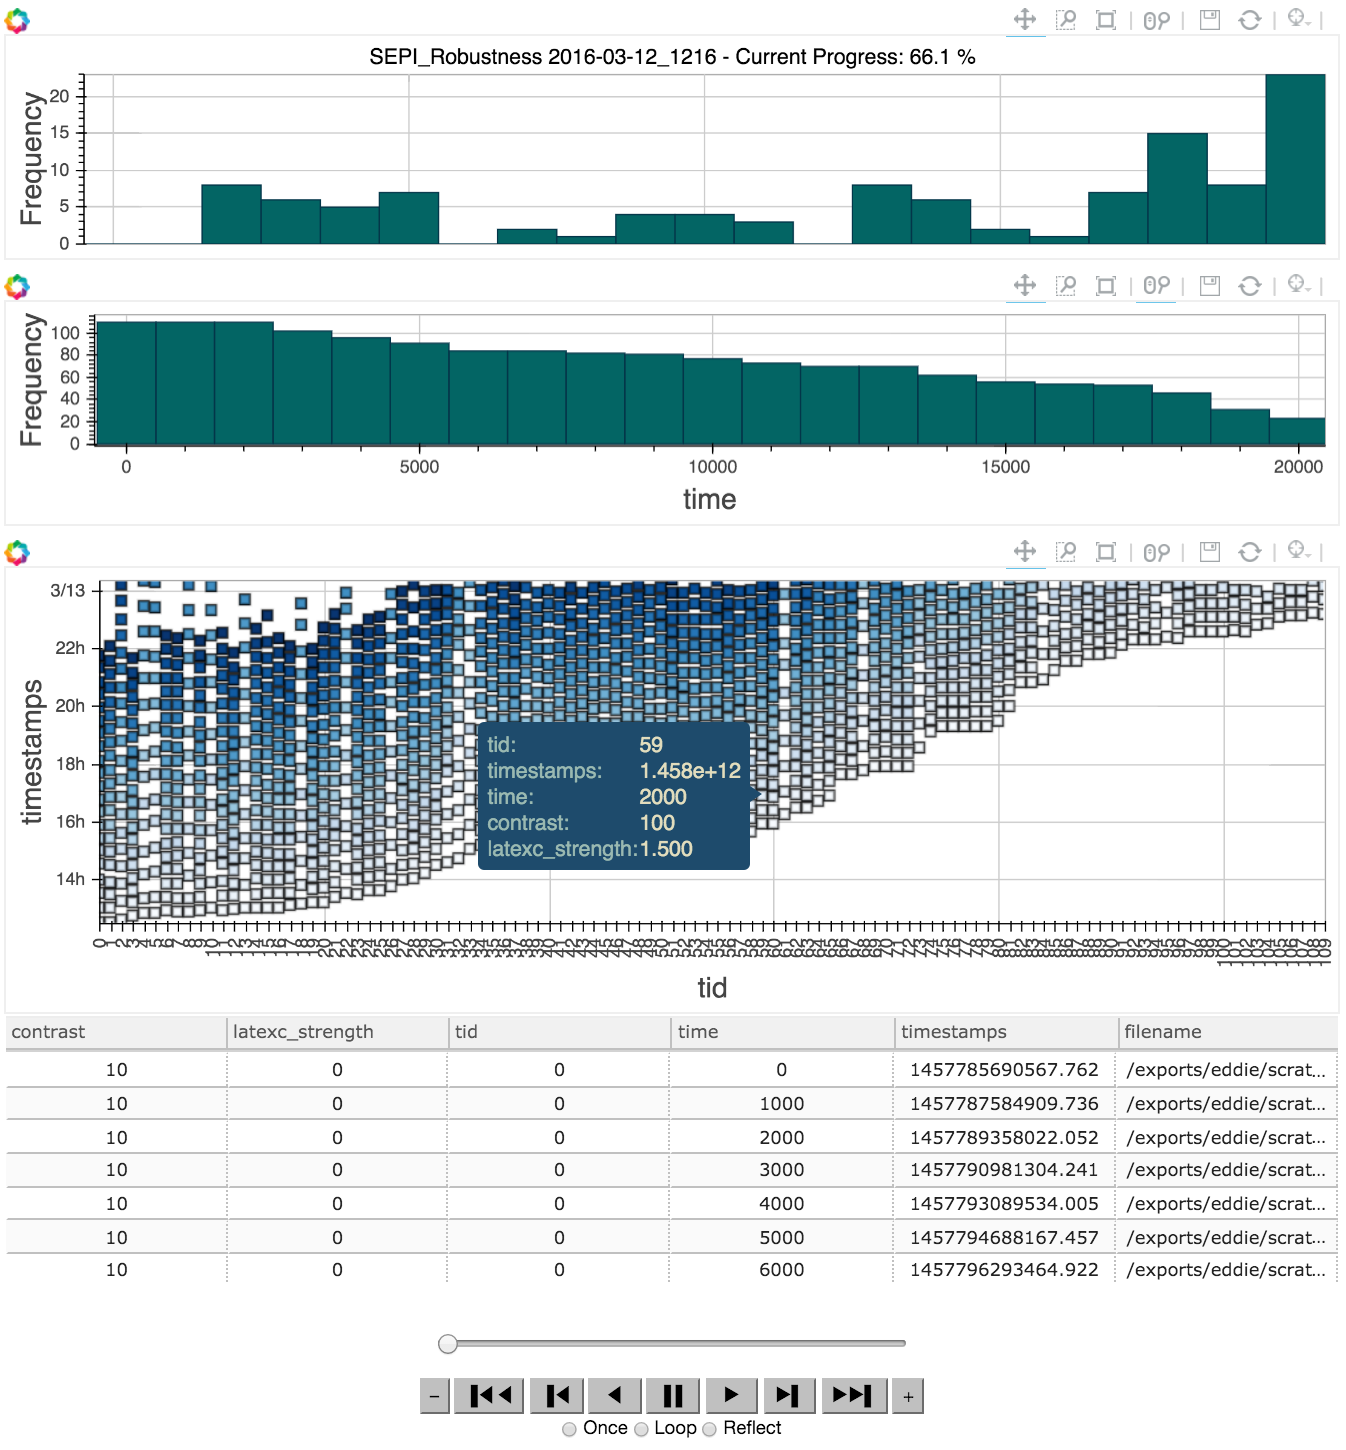
\includegraphics[width=1.0\textwidth]{workflow_progress.png}
	    \caption[Interactive dashboard to monitor workflow
          progress.]{Interactive real time dashboard to monitor the
          progress of an experiment and catch any problems or failures
          in individual jobs. Top panel shows current progress in
          developmental time, second panel shows completion at each
          time. Third panel plots the times at which each part of a
          job completed.}
	\label{workflow_progress}
\end{figure}


\subsection{Step 5: Loading results}

A core part of the workflow is linking up the output generated by
Lancet with the data structures provided by HoloViews. In order to
make this easy the user can specify a file pattern to search for
generated files, which can be loaded into a Table. The Table can then
be expanded into another HoloViews data structure called a Layout,
which makes it possible to access individual measurements or analyses
without having to load the whole file. This means that with just a
single line of code we can specify precisely which measurement and
which part of the parameter space to load, then visualize it immediately
using interactive widgets and complex plot arrangements.

Each measurement or analysis can be accessed via a tree-like
structure, letting us access individual measurements by accessing them
with attribute access and selecting by the parameter values.

\begin{minipage}{\linewidth}
\begin{lstlisting}
  :Layout
   .CFs.LateralInhibitory     :Collator   [Index,contrast,latexc_strength,tid,time,timestamps]   (filename,entries)
   .CFs.LateralExcitatory     :Collator   [Index,contrast,latexc_strength,tid,time,timestamps]   (filename,entries)
   .OrientationPreference.V1  :Collator   [Index,contrast,latexc_strength,tid,time,timestamps]   (filename,entries)
   .OrientationSelectivity.V1 :Collator   [Index,contrast,latexc_strength,tid,time,timestamps]   (filename,entries)
\end{lstlisting}
\end{minipage}


\begin{figure}
	\centering
        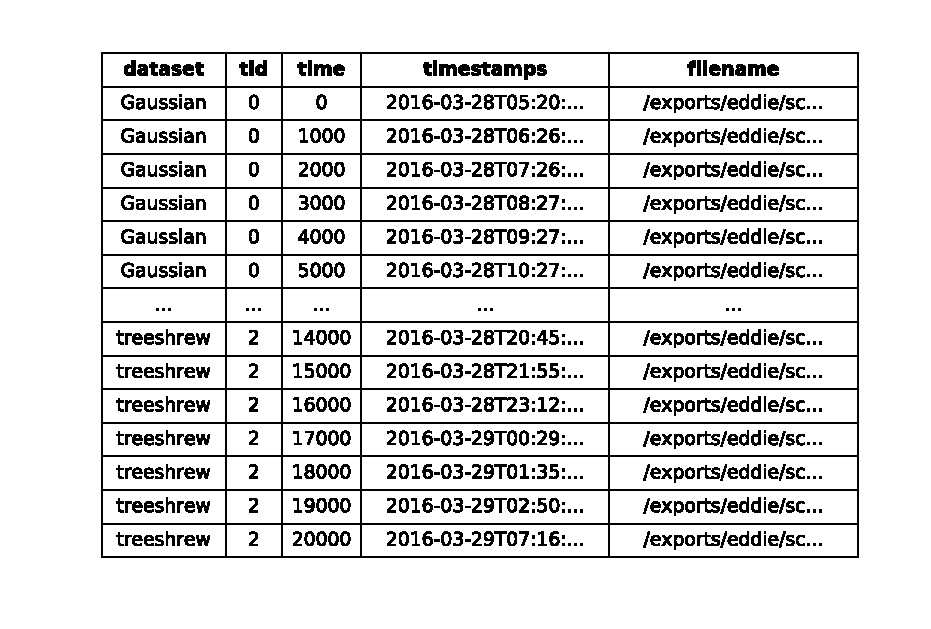
\includegraphics[width=0.7\textwidth]{workflow_load.pdf}
	    \caption[Table summarizing results from parameter analysis in
          Lancet and HoloViews.]{Table showing the output of a
          parameter exploration using Lancet and HoloViews. Each row
          represents one file of measurement results. The Table allows
          selecting just the subset of files to be loaded.}
	\label{workflow_load}
\end{figure}


\subsection{Step 6: Analysis and Visualization}

The exploratory analysis and visualization of a dataset is one of the
most important aspect of a scientist's workflow. However, traditional
analysis and visualization libraries split those two aspects apart,
which provides a significant bottleneck to what the user actually
wants to do, namely to understand their data. By giving data elements
their own visual representation, we can provide immediate visual
feedback, while still making all the data available for further
numerical processing. HoloViews also provides containers and other
datastructures that automatically get translated into complex and powerful plot
arrangements and widgets, making it trivial to explore datasets of any
dimensionality and complexity.

In the previous step we saw how to load a dataset.  Here we will
quickly demonstrate how we can work with this data once it is loaded.
As an example we load some of the weights that represent synaptic
neural connections between different neurons in our model. In
Figure~\ref{workflow_explore} we can see how we can load two sets of
weights for a specific set of parameters and compose them together by
overlaying them. The resulting visualization demonstrates the
complexity this approach allows as we can represent the X/Y positions
of the neurons in the V1 sheet on a grid, while representing other
dimensions such as the lateral excitatory strength and contrast as
sliders. Such a plot would usually be very complex to construct, but
here it is just a side-effect of the way the data has been structured
and annotated and we could easily transform the dataset to slice and
visualize it in any number of ways. Furthermore all the underlying
weights are easily accessible and we can therefore feed this data
structure straight into further analysis functions.

Combining visualization and analysis in this proves to be an
incredibly powerful paradigm to work with large datasets. The main
benefits are that the user no longer has to manually keep track of
metadata, which means that plots automatically generate appropriate
labels and the analysis code always has access to all the information
it requires. This also means that instead of storing a plot in an
unreproducible format, the full specification of the plot including
data, metadata, and styling details can be stored as a single object,
which can be loaded later to extract the raw data or merely to
reproduce the plot.

\begin{figure}
	\centering
        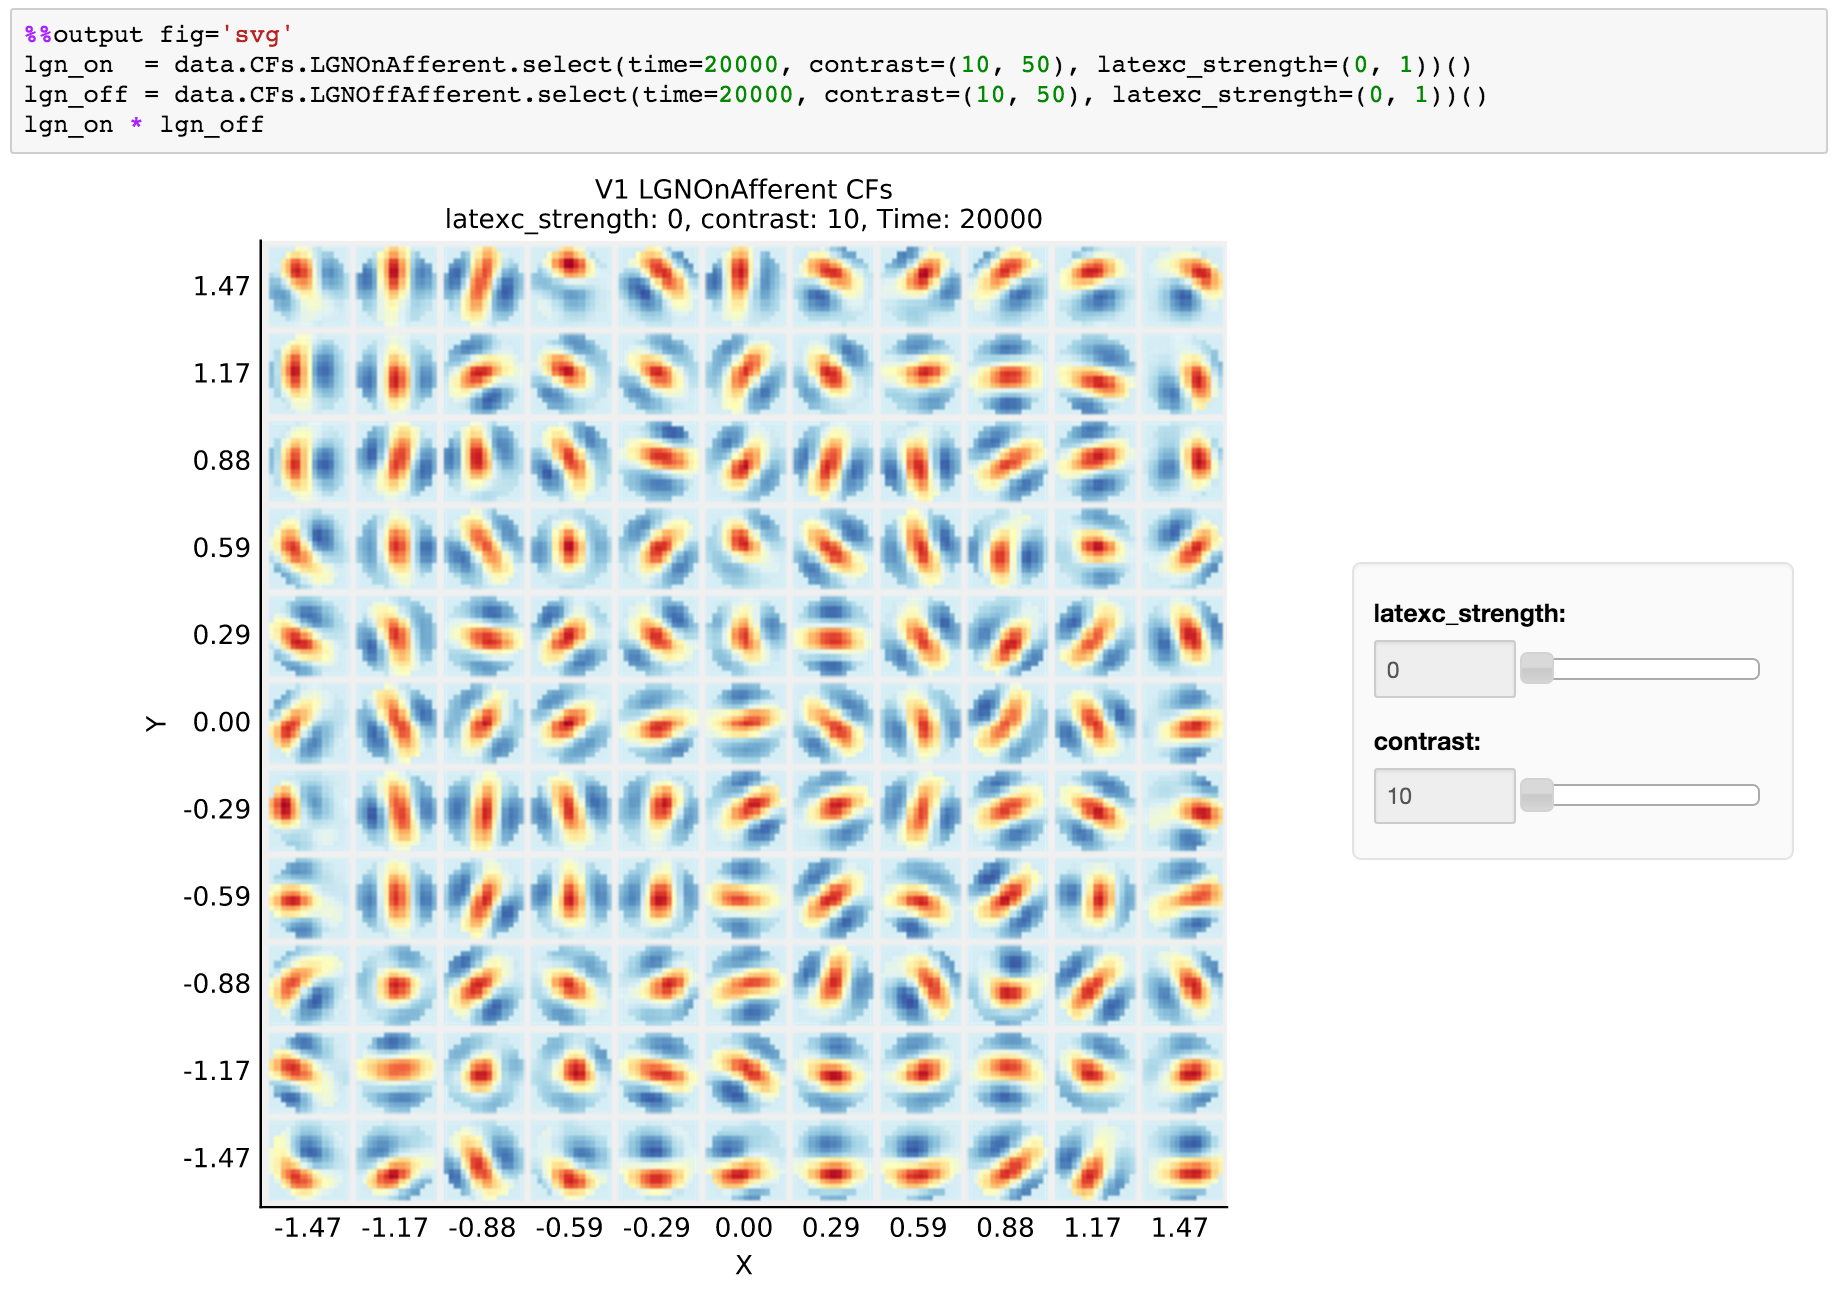
\includegraphics[width=1.0\textwidth]{workflow_explore.png}
	\caption[Demonstration of complex parameter exploration in
      HoloViews.]{Demonstration of loading a measurement from the
      parameter exploration showing the afferent weights of the model
      varying across the parameter space we defined for the
      experiment. Through the use of multi-dimensional datastructures
      we can achieve complex plotting arrangements and explore any
      further data dimensions using widgets, which appear
      automatically.}
	\label{workflow_explore}
\end{figure}

\subsection{Step 7: Visual aesthetics and publication-quality plotting}

The flexibility of HoloViews not only allows for quick data
exploration but even extends to generating publication-quality
figures. As stated previously, all plots used as part of this thesis
were generated using HoloViews and each chapter is accompanied by
notebooks, which replicate the entire workflow. This is made possible
because HoloViews allows for huge flexibility in customizing the
automatically generated visual representations.

\section{Summary}

In this chapter we have demonstrated a complete workflow for the
specification, launching, collection, exploration and visualization of
a computational experiment developed for this thesis. It provides huge
benefits in terms of usability and reproducibility over previous
approaches, since it captures the full breadth of an individual
research project, keeping a complete record of everything required to
reproduce both the data and the actual published figures.  It is
already in use for research projects ranging from
neuroscience \citep{Keemink2015} to physics \citep{Nijholt2015,
  Tenner2016}, astronomy, meteorology, and chemistry.

